%!TEX root=../GaugeCNNTheory.tex


\subsubsection*{هموردایی دورانی سراسری روی $\Euc_2 \backslash \{0\}$}
\label{sec:polar_Euc2_rot}

ما با مدل‌های مفهومی ساده‌تر شروع می‌کنیم، که شبکه‌های هموردای دورانی سراسری هستند و تنها بر $\{e\}$-ساختارهای ناوردای دورانی روی~$\Euc_2 \backslash \{0\}$ تکیه دارند~\cite{finzi2020generalizing,chidester2019rotation}.
این مدل‌ها متریک اقلیدسی استاندارد را روی~$\Euc_2 \backslash \{0\}$ فرض می‌کنند، که نسبت به آن چارچوب‌ها راست‌هنجار هستند.
در مجموع، این دو الزام به $\{e\}$-ساختارهایی منجر می‌شوند که در شکل~\ref{fig:G_structures_R2_no_origin} نشان داده شده‌اند.

علاوه بر $G$-ساختارهای در نظر گرفته شده، شبکه‌ها به پیاده‌سازی خاص پول‌بک انتقال‌دهنده و در نتیجه به ژئودزیک‌ها و انتقال‌دهنده‌های موازی بستگی دارند.
ژئودزیک‌ها در هر دو مدل، ژئودزیک‌های استاندارد در فضاهای اقلیدسی (یعنی خطوط مستقیم) فرض می‌شوند، که متناظر با اتصال لوی-چیویتا از متریک اقلیدسی است.
از آنجا که $\Euc_2 \backslash \{0\}$ از نظر ژئودزیکی کامل نیست، برای نگاشت‌های نمایی که در مبدأ به پایان می‌رسند، باید از پدینگ-صفر استفاده شود.
توجه داشته باشید که این امر تأثیری بر نتیجه نهایی ندارد زیرا ژئودزیک‌های از دست رفته دارای اندازه صفر هستند.


از سوی دیگر، انتقال موازی بردارهای ویژگی، با اتصال لوی-چیویتا مطابقت \emph{ندارد} زیرا اتصال لوی-چیویتا با $\{e\}$-ساختارها سازگار نیست.
در عوض، مدل‌ها \emph{اتصالات بدیهی} یکتای $\{e\}$-سازگار را فرض می‌کنند که توسط $\{e\}$-ساختارهای مربوطه القا می‌شوند.%
\footnote{
\label{footnote:punctured_Euclidean_transport}
	انیمیشنی از انتقال $\{e\}$-سازگار متناظر با شکل~\ref{fig:G_structure_R2_no_origin_SO2} را می‌توان در
	\href{https://en.wikipedia.org/wiki/Levi-Civita_connection\#Parallel_transport}{\underline{ویکی‌پدیا}} یافت.
}
مطابق با اتصالات بدیهی، ضرایب عددی بردارهای ویژگی هنگام انتقال، تبدیل نمی‌شوند، علی‌رغم اینکه چارچوب‌ها نسبت به مفهوم معمول توازی در فضاهای اقلیدسی چرخانده می‌شوند.
در عمل، این فقط به این معنی است که انتقال‌دهنده‌های $\rho(g^{A\widetilde{A}}_\gamma) = \id_{\R^c}$ را می‌توان در پیاده‌سازی نادیده گرفت -- که دلیلی است که آنها در مقالات اصلی مورد بحث قرار نگرفته‌اند~\cite{finzi2020generalizing,chidester2019rotation}.


از آنجا که دوران‌ها $\{e\}$-ساختارهای در نظر گرفته شده را ناوردا باقی می‌گذارند و در عین حال ایزومتری هستند، ما داریم
$\IsomeM = \SO2$ برای مدل \citet{finzi2020generalizing} (شکل~\ref{fig:G_structure_R2_no_origin_SO2}) و
$\IsomeM = \operatorname{C}_8$ برای مدل \citet{chidester2019rotation} (شکل~\ref{fig:G_structure_R2_no_origin_C8}).
قضیه~\ref{thm:isom_equiv_GM_conv} سپس تأیید می‌کند که کانولوشن‌های $\GM$ متناظر، $\IsomeM$-هموردا هستند، که با گزاره‌های بیان شده توسط نویسندگان مطابقت دارد.

\begin{SCfigure}
	\centering
	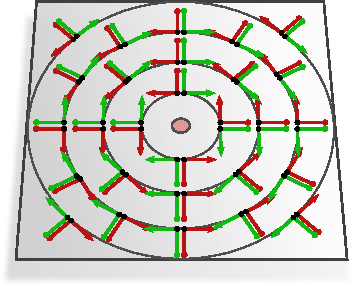
\includegraphics[width=.34\textwidth]{figures/G_structure_R2_no_origin_O2.pdf}
	\hspace*{2.ex}
	\captionsetup{width=.92\textwidth}
	\caption{\small
		یک $\Flip$-ساختار $\OO2$-ناوردا روی $\Euc_2 \backslash \{0\}$، که با افزودن نسخه‌های بازتابیده به هر چارچوب از $\{e\}$-ساختار در شکل~\ref{fig:G_structure_R2_no_origin_SO2} ساخته شده است.
		کانولوشن $\GM$ متناظر به طور همزمان نسبت به دوران‌ها و بازتاب‌های سراسری در $\IsomRM = \OO2$ حول مبدأ هموردا است.
		\\\protect\rule{0ex}{5.5ex}
	}
	\label{fig:G_structure_R2_no_origin_O2}
\end{SCfigure}


قبل از ادامه می‌خواهیم اشاره کنیم که $\{e\}$-ساختار $\operatorname{C}_8$-ناوردا در شکل~\ref{fig:G_structure_R2_no_origin_C8} پیوسته نیست و بنابراین استنتاج پیوسته (یا هموار) را تضمین نمی‌کند.
یک مزیت این $\{e\}$-ساختار از دیدگاه مهندسی این است که به صورت محلی با $\{e\}$-ساختار کانونی $\R^2$ ایزومتریک است، که اجازه می‌دهد روال‌های کانولوشن اقلیدسی متعارف روی هر هشتک اجرا شوند.
نویسندگان تعمیم به $\{e\}$-ساختارهای $\CN$-ناوردا را مورد بحث قرار می‌دهند، که در حد $N\to\infty$ معادل $\{e\}$-ساختار $\SO2$-ناوردا در شکل~\ref{fig:G_structure_R2_no_origin_SO2} می‌شوند.

علاوه بر این، با استفاده از کرنل‌های راهبری‌پذیر بازتابی به جای کرنل‌های نامحدود، می‌توان مدل‌ها را به صورت سراسری $\OO2$-هموردا ساخت.
از دیدگاه نظری، این متناظر با $\Flip$-ساختار $\RM$ ناوردای $\IsomRM = \OO2$ روی $\Euc_2 \backslash \{0\}$ است که در شکل~\ref{fig:G_structure_R2_no_origin_O2} نشان داده شده است.
توجه داشته باشید که $\RM$ یک کلاف $\Flip$ روی $\Euc_2 \backslash \{0\}$ است، که تحدید آن به دایره‌هایی با شعاع ثابت، به عنوان یک کلاف اصلی، با $\OO2$ که به عنوان یک کلاف $\Flip$ روی فضای خارج‌قسمتی $\OO2/\Flip \cong S^1$ تفسیر می‌شود، ایزومورف است.